\title{Syntax and Semantics Exam}
\author{
        Benjamin Bennetzen \\
        Student ID: 20204861 \\
        Computer Science, 4th semester\\
}
\date{\today}

\documentclass[12pt]{article}

\usepackage{tikz}
\usepackage{listings}
\usepackage{mathpartir}
\usepackage{ebproof}
\usepackage{amsmath}
\usepackage[utf8]{inputenc}
\usepackage{amssymb}
\usepackage{graphicx}
\usepackage{stmaryrd}

\newcommand{\R}{\mathbb{R}}
\newcommand{\F}{\mathbb{F}}
\newcommand{\num}[1]{\mathcal{N}\llbracket #1 \rrbracket}
\newcommand{\ul}[1]{\underline{#1}}

\begin{document}
\maketitle

\section{Exercise 1}
\subsection{}
\begin{itemize}
        \item A $a \cup b \cup c$: is automata ii.
        \item B $\Sigma^*$: automata iv.
        \item C $a^* \cup b^* \cup c^*$: automata iii.
        \item D $(a \cup b)^* \cup c^*$: automata i.
\end{itemize}

\subsection{}
\begin{itemize}
        \item The union of two regular languages is regular: Yes.
        \item The union of twe context-free languages is context-free: Yes.
        \item Assuming the language L is recognized by the NFA $(Q, \Sigma, \delta, q_0, F)$, a possible pumping length for language L would be $p=$: When using the pumping lemma the length of the word has depend on $p$, however any value bigger than or equal to $p$ will do.
\end{itemize}

\section{Exercise 2}
\subsection{}
In state 2 we can notice that that when we read a $b$ from the input it does not depend on what is in the stack, and we also push a $b$ onto the stack. When we read an $a$ from the input we always have to have a $b$ on the stack meaning that at some point before this we should have already read a $b$. Lastly we should notice that the stack has to be emptied before we can enter the accepting state. This leads me to the following definition for the language $L = \{w \in \Sigma^* \mid |w|_a = |w|_b, |w'|_a \leq |w'|_b\}$, where $w'$ is a prefix of $w$. This means that in the final word there has to be as many $a$'s as there are $b$'s, but in any given prefix of the word there can be more $b$'s than $a$'s.

\subsection{}
No, the CFG and the PDA do not describe the same language. This can be shown with the word $b$.

Using the CFG we can derive the word as follows. $S \Rightarrow Sb \Rightarrow \epsilon b$.

However, the PDA will not accapt this word. $1[] \rightarrow_{\epsilon,\epsilon} 2[\$] \rightarrow_{b,\epsilon} 2[b\$]$. We end in a situation where we have a $b$ on the stack, but not more input. Therefore we end in state 2, which is not an accepting state.

\section{Exercise 3}
Proof by contradiction. We Assume that $L$ is regular. By the pumping lemma we know that there exits a pumping length $p \geq 1$ such that for every $w \in L$, where $|w| \geq p$ then there exits a decomposition $w = xyz$, such that.

\begin{enumerate}
        \item for all $i \geq 0$, $xy^iz \in L$
        \item $|y| > 0$
        \item $|xy| \leq p$
\end{enumerate}

We choose the word $a^{p^3}$, The word is clearly both in $L$ and length at least $p$. From condition 2  and 3 we know that $y=a^k$ where $1 \leq k \leq p$ When we pump with $i=2$ we get the following word $a^{p^3 + k}$. Given the constraints on $k$, $p^3 + k$ cannot be written in the form $n^3$, where $n=p+1$. Therefore $a^{p^3 + k} \notin L$, thus we cannot satisfy condition 1.

\section{Exercise 4}
\subsection{}
To prove the two statements i will provide a proof tree for each of them.

First the proof tree for $ab \rightarrow 2$

\begin{center}
\begin{prooftree}
        \infer0[by rule 2]{b \rightarrow 2}
        \infer1[$3 = 2 + 1$, by rule 3]{ab \rightarrow 3}
\end{prooftree}
\end{center}

Then the prooftree for $aab \rightarrow 4$.

\begin{center}
\begin{prooftree}
        \infer0[by rule 2]{b \rightarrow 2}
        \infer1[$3 = 2 + 1$, by rule 3]{ab \rightarrow 3}
        \infer1[$4 = 3 + 1$, by rule 3]{aab \rightarrow 4}
\end{prooftree}
\end{center}

\subsection{}
First we show thet the property holds for our base case which given that $L' = \{a,b\}^+$, means the words of length 1, those being $a$ and $b$. From rule 1 we know that $a \rightarrow 1$, which upholds the property as $|a|_a + 2|a|_b = 1$. For the word $b$, we know from rule 2 that $b \rightarrow 2$ which again upholds the property as $|b|_a + 2|b|_b = 2$.

For the induction step we have  words of length $n + 1$. We can divide these words into two cases $aw$ and $bw$, where $w$ is some word of length $n$. For the case of $aw$ we have to use rule 3. By our induction hypothesis we know that $w$ upholds the property. For the word $aw$ to uphold the property it the resulting value has to be one bigger than the resulting value of $w$ as there is one more $a$. In rule 3 that exactly what we do $aw \rightarrow k'$, where $k' = k + 1$ and $k$ is the resulting value of $w$. For the word $bw$ the same arguments can be, but to uphold the property 2 has to be added to the resulting value of $w$. In rule 4 we can see that $bw \rightarrow k'$, where $k' = k + 2$ and $k$ is the resulting value of $w$, therefore we have that both cases uphold the property.

\section{Exercise 5}
\subsection{}
With fully static scoping we can make the bindings as seen in Figure \ref{fig:static}. With these bindings $y=3$.

\begin{figure}[h!]
        \centering
        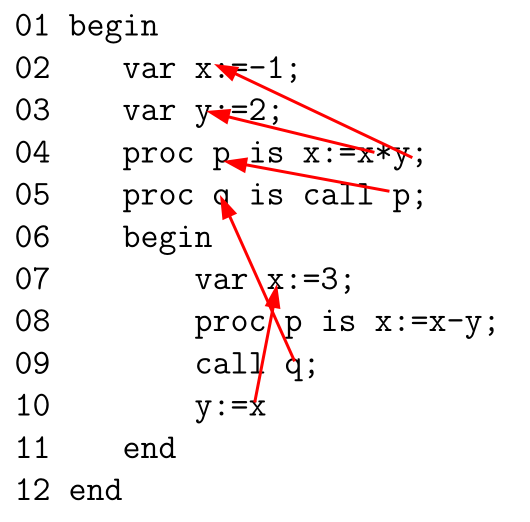
\includegraphics[width=0.5\textwidth]{static.png}
        \caption{Fully static scope bindings.}
        \label{fig:static}
\end{figure}

\subsection{}
With fully dynamic scoping we can make the bindings as seen in Figure \ref{fig:dynamic}. With these bindings $y=1$.

\begin{figure}[h!]
        \centering
        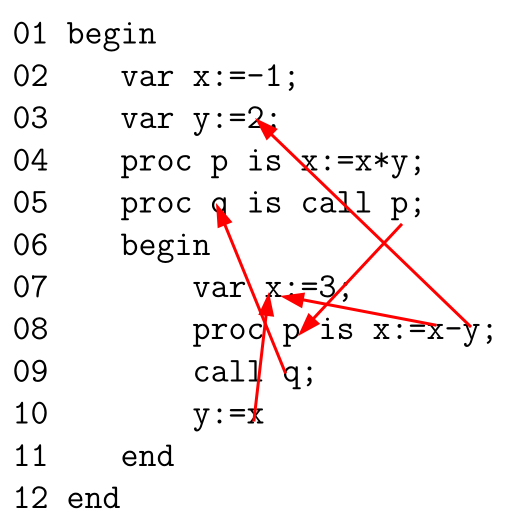
\includegraphics[width=0.5\textwidth]{dynamic.png}
        \caption{Fully dynamic scope bindings.}
        \label{fig:dynamic}
\end{figure}

\subsection{}
With the static scoping for procedures and dynamic scoping for variables we can make the bindings as seen in Figure \ref{fig:mixed}. With these bindings $y=6$.

\begin{figure}[h!]
        \centering
        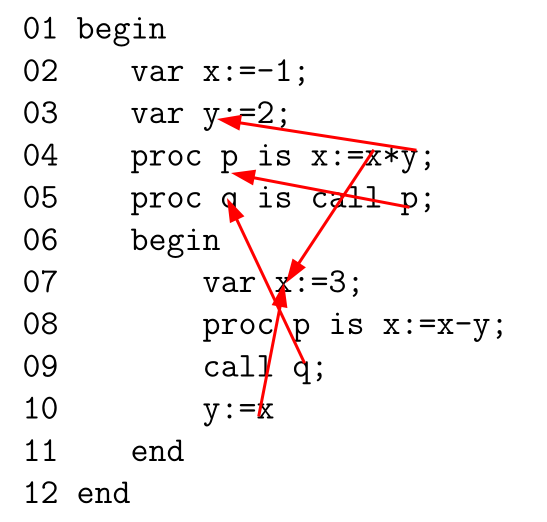
\includegraphics[width=0.5\textwidth]{mixed.png}
        \caption{Mixed scope rules.}
        \label{fig:mixed}
\end{figure}

\end{document}
